\section{Design}\label{sec:design}

\begin{figure}
  \centering
  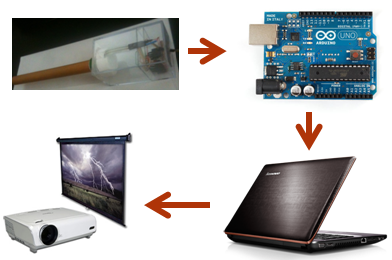
\includegraphics[width=0.8\linewidth]{./figs/sketch.png}
  \caption{Overview of how our system works.}
  \label{fig:design-sketch}
\end{figure}

To increase the intuitiveness of our system, we build the device to look as natural as possible. We tried to make sure that users will understand what to do with the tube and how to use it at the first time they see it, without any special instruction. We also designed our system to be more persistence so that users will not only stay for five minutes to explore what they can do; we want them to be addicted to the games and application.

The first approach that we did to increase the user intuitiveness and user’s persistence is to make the mouth piece of the device to appear similar to a blowgun so that users will know immediately that they need to blow. We also add a spectrum circle in front of the mouth piece to let the user know that rotating the device will change the color. Last but not least, we also plan to create multiple applications and games that can be control with the tube so that users will not be bored easily and will keep on testing the unlimited possibilities on what they can do with the tube.

